\documentclass[11pt, a4paper]{article}
\usepackage[a4paper, total={6.5 in,9in}]{geometry}
\usepackage[slovene]{babel}
\usepackage[utf8]{inputenc}
\usepackage[T1]{fontenc}
\usepackage{lmodern}
\usepackage{amsmath}
\usepackage{ amssymb }
\usepackage{amsfonts}
\usepackage{amsthm}
\usepackage{url}
\usepackage{gensymb}
\usepackage{subcaption}
\usepackage[pdftex]{graphicx}
\usepackage[section]{placeins}
\usepackage{mathtools}
\usepackage{float}
\usepackage{epstopdf}
\renewcommand{\vec}[1]{\mathbf{#1}}
\usepackage{hyperref}
\usepackage{wrapfig}
\usepackage{pdfpages}
\pagestyle{plain}

\begin{document}
	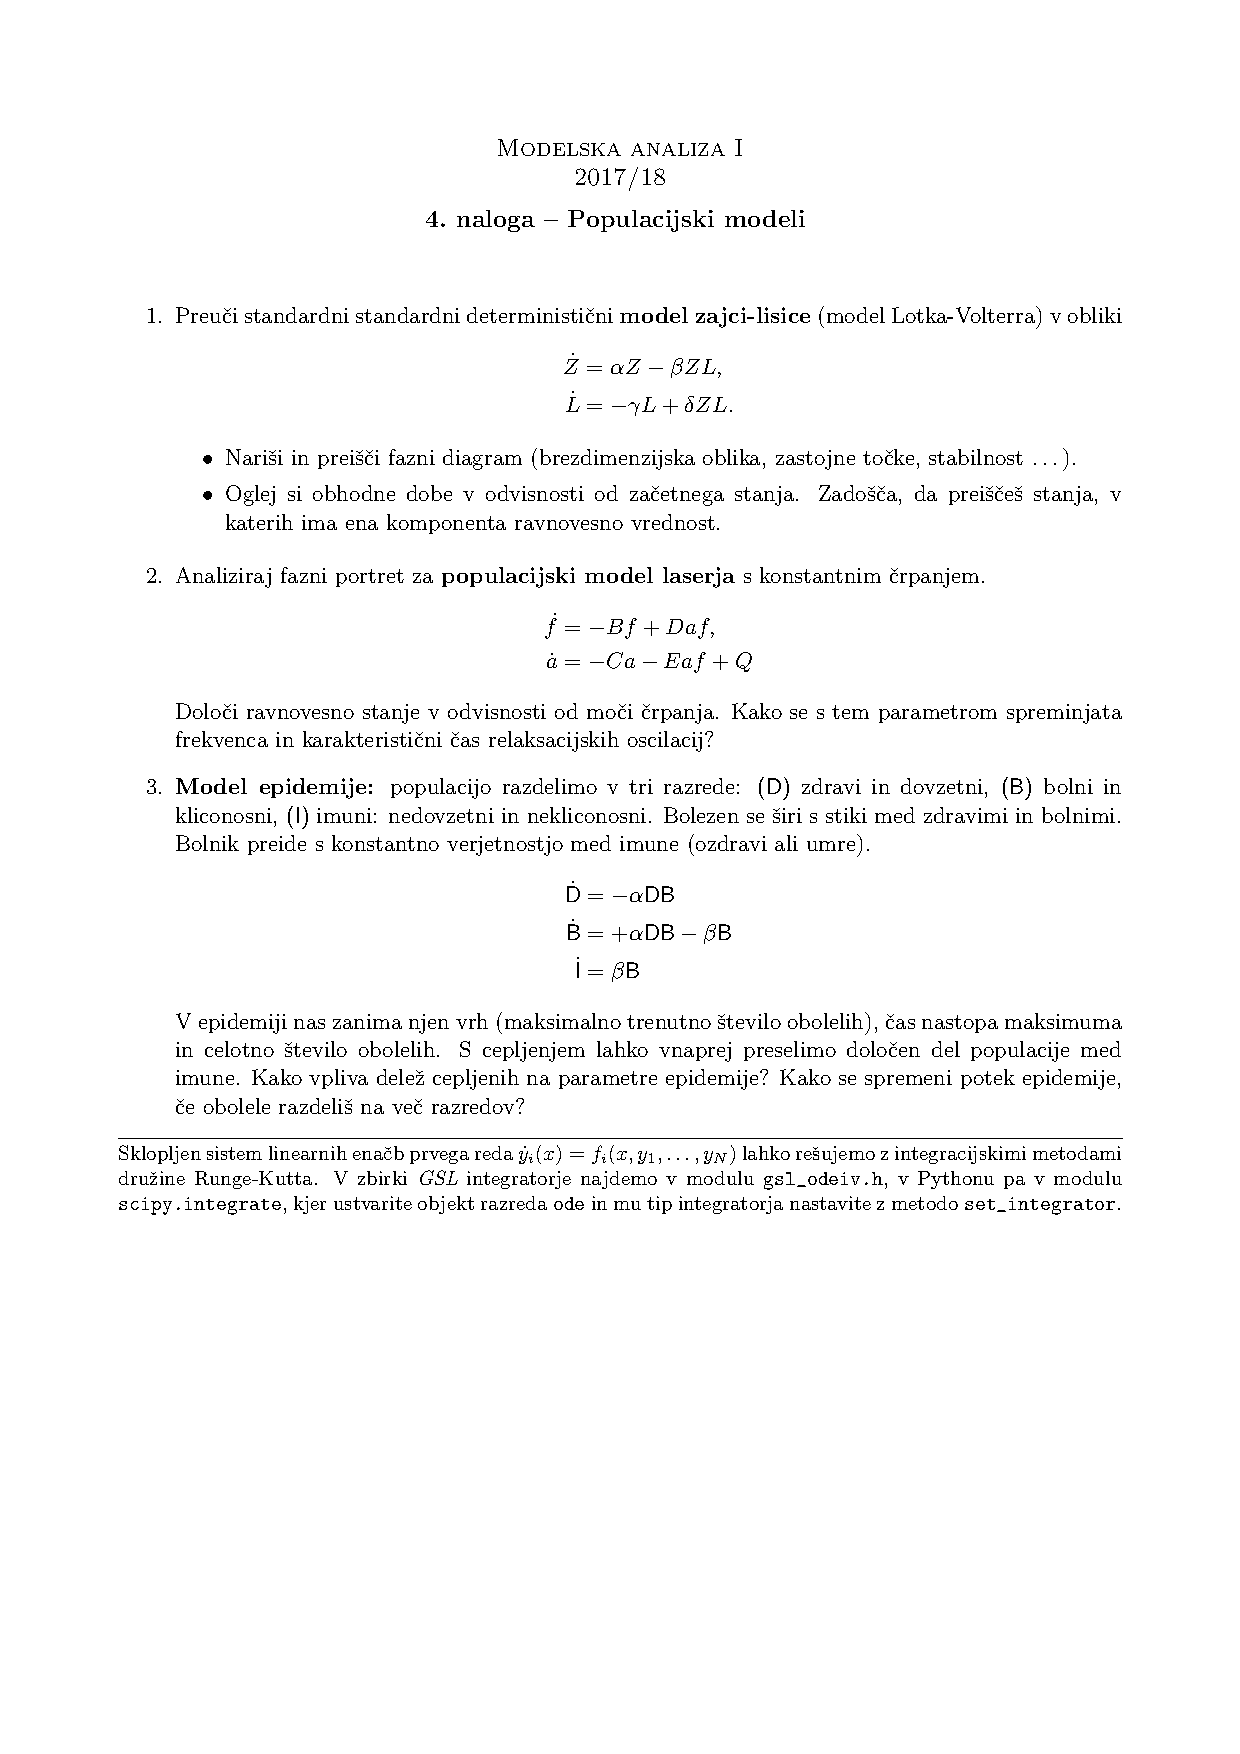
\includepdf[pages={1}]{mod104.pdf}
	\begin{center}
	{\LARGE\bfseries 4. naloga - populacijski modeli \par}
	\vspace{1cm}
	
	{\Large Domača naloga pri predmetu Modelska analiza I\par}
	\vspace{0.2cm}
	{\normalsize Avtor: Matic Noč \par}
	\vspace{0.2cm}	
	{\normalsize 17.10.2017 \par}	

	

	
	\end{center}

\section{Uvod}
Obravnavali bomo populacijske modele, ki jih lahko modeliramo s sklopljenimi diferencialnimi enačbami prvega reda. Seveda je rešitev enačb močno odvisna od začetnih pogojev, tako bomo pri epidemiji dobili različne razmahe epidemij, pri populaciji zajcev in lisic, različne dobe periodičnega vzpona populacije in pri laserjih različne relaksacijske konstante laserja.

\section{Epidemija}
Epidemijo lahko opišemo s sistemom diferencialnih enačb, kjer populacijo razdelimo v tri razrede: (D) zdravi in dovzetni, (B) bolni in (I) imuni oziroma pokončani. Gre za logistični model.
\begin{equation}
\begin{array} {lcl} \dot{D} & = & -\alpha DB \\
\dot{B}  & = & +\alpha DB - \beta B 
 \\
\dot{I}  & = & +\beta B \end{array}
\end{equation}
 Problema se lotimo numerično s metodo Runge - Kutta in dobimo rešitve za D(t), B(t) in I(t).
Poglejmo si zanimivosti rešitev.
\begin{figure}[htb!]
  \centering
  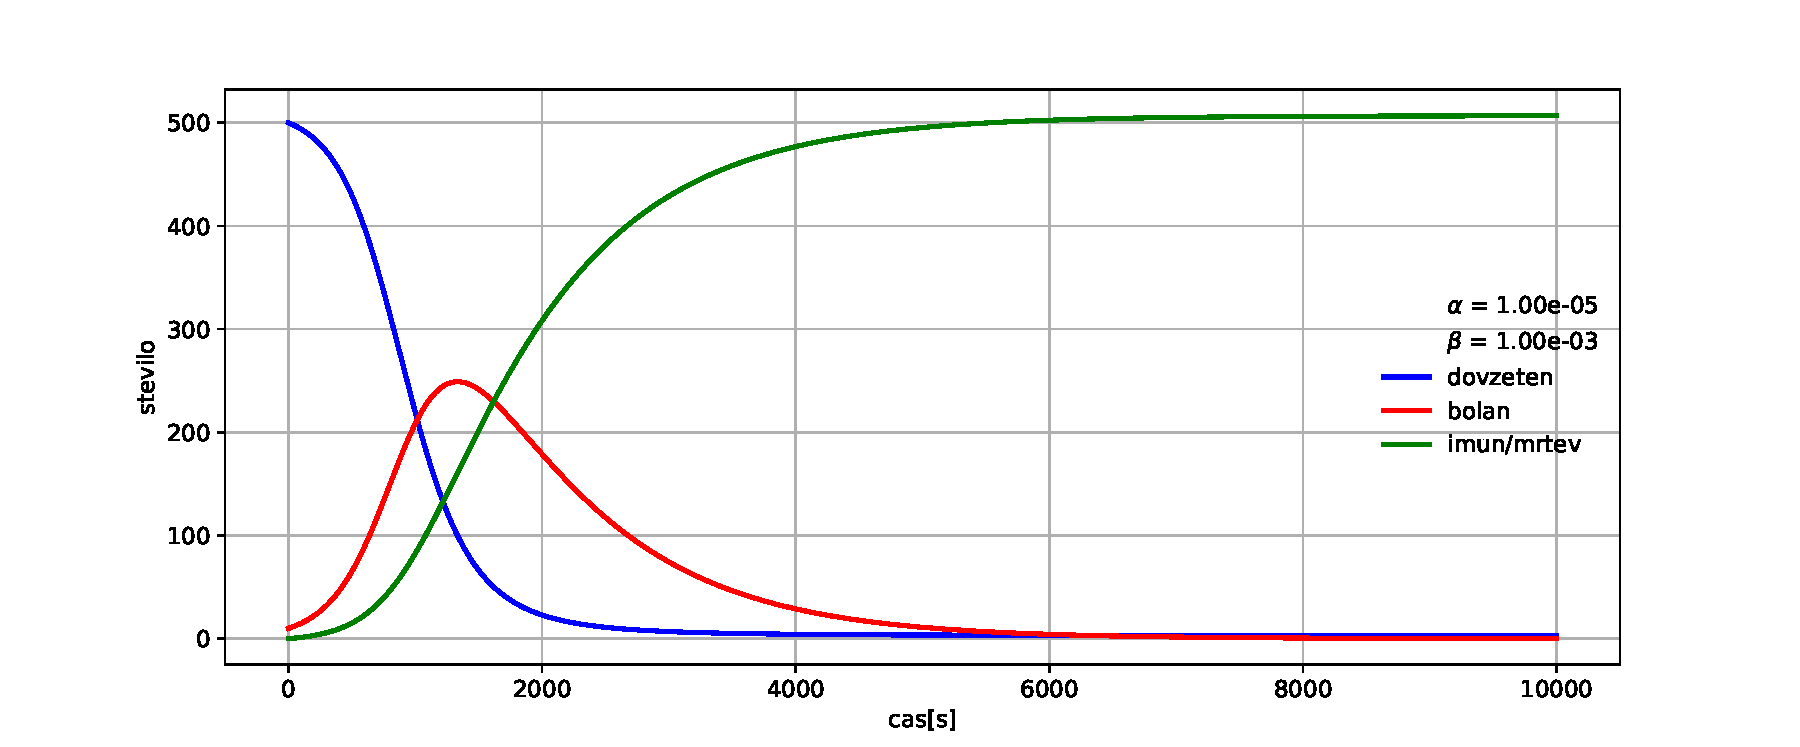
\includegraphics[width=18cm]{oblika_grafa.pdf}
 \caption{Osnovna rešitev logističnih enačb nam da rešitev razmaha epidemije, na začetku imamo 500 dovzetnih, ki nato postanejo imuni/mrtvi.}
\end{figure}
\subsection{Nižanje vrha epidemije}
Ko zmanjšujemo konstanto $\alpha$, ki pomeni pogostost srečanja D in B, se vrh epidemije pojavi kasneje in je zaradi večjega trajanja prehajanja bolnih med imune tudi manjši.
\begin{figure}[htb!]
  \centering
  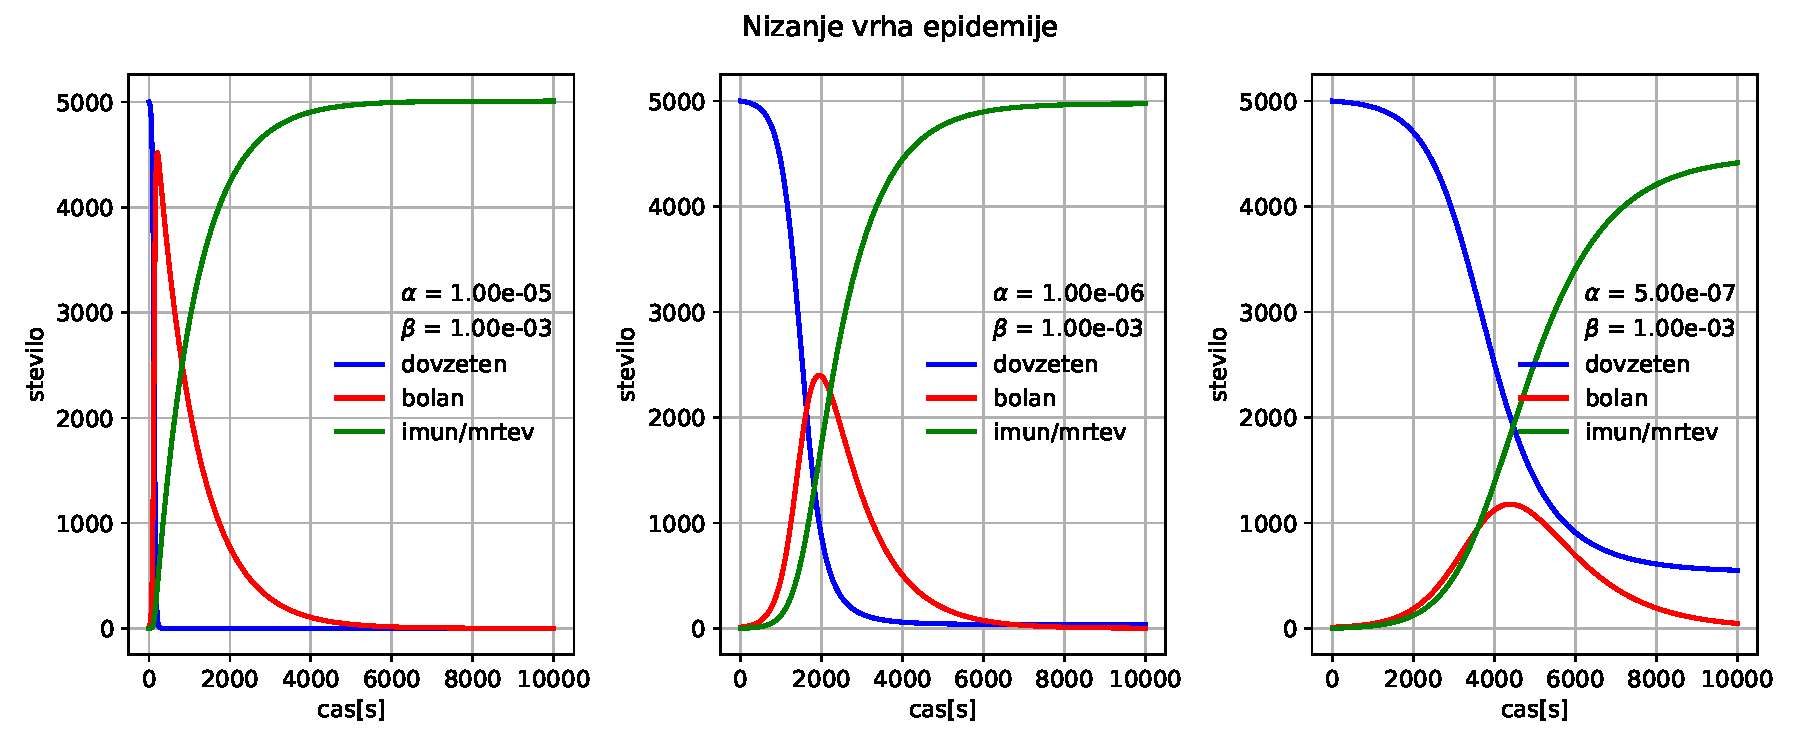
\includegraphics[width=18cm]{nizanje_vrha_zaradi_alfa.pdf}
  \caption{Nižanje vrha epidemije zaradi manjšega srečanja bolnih in dovzetnih}
\end{figure}
\subsection{Cepljenje ljudi}
Koliko ljudi moramo cepiti, da preprečimo razmah epdimije? Odgovor lahko dobimo če postavimo začetne pogoje za imune iz 0 na določen delež prebivalcev.
\begin{figure}[htb!]
  \centering
  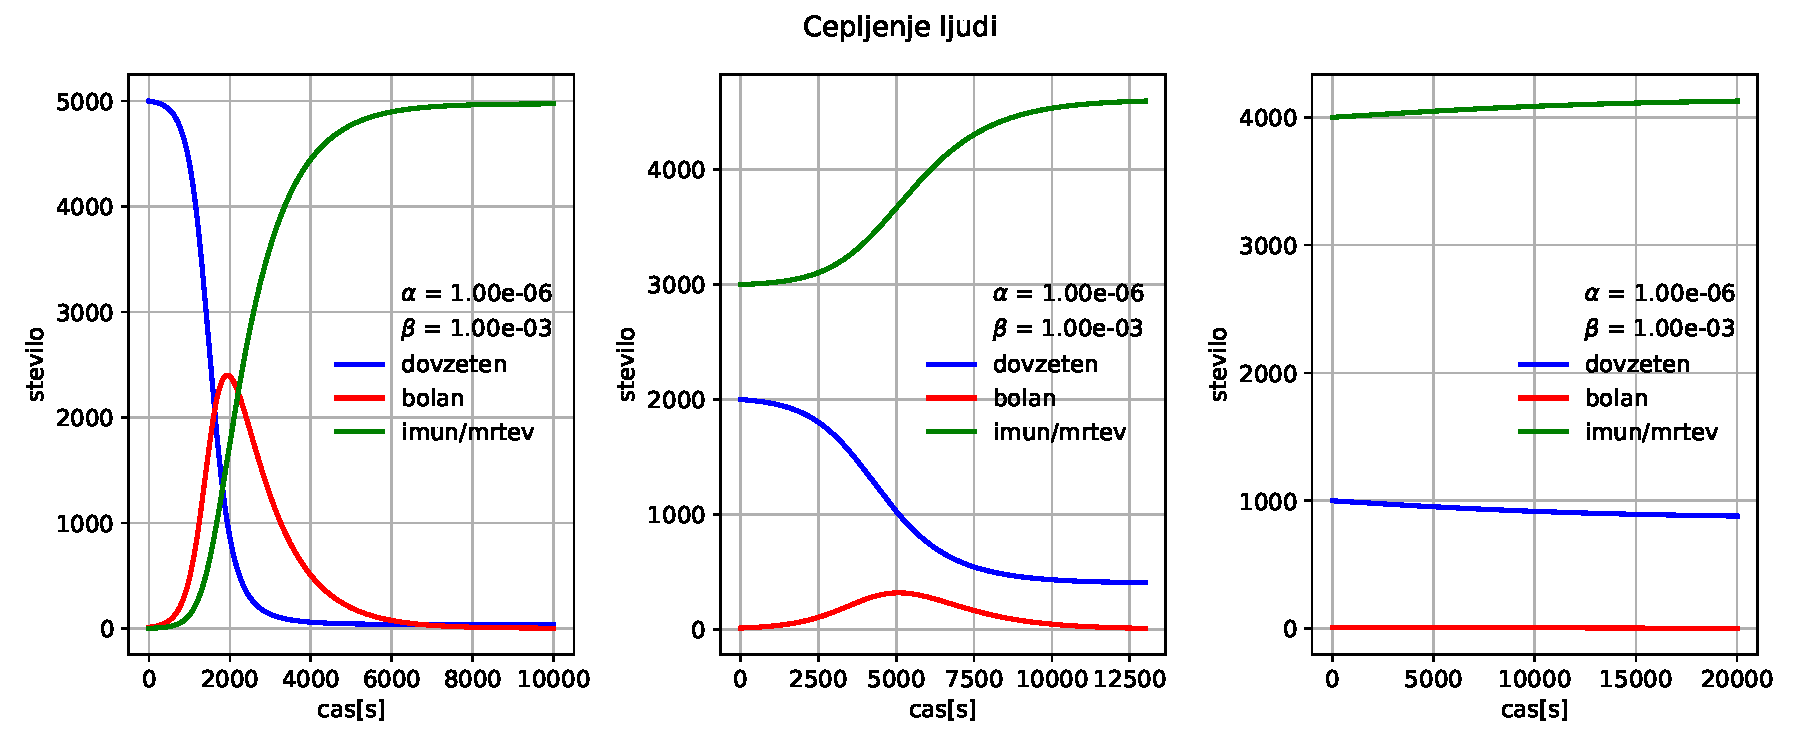
\includegraphics[width=18cm]{cepljenje_ljudi.pdf}
  \caption{Vidimo da se je že pri cepitvi 3/5 ljudi epidemija močno zmanjšala, pri cepitvi 4/5 ljudi pa do epidemije sploh ne pride, eksponentno počasi postajajo ljudi bolni in bolni imuni.}
\end{figure}
\subsection{Več stopenj bolezni}
Recimo, da se bolezen začne s kašljanjem, nato pa preide vsakič v novo stopnjo. Za tak opis epidemije lahko razširimo enačbe (1)
\begin{equation}
\begin{array} {lcl} \dot{D} & = & -\alpha DB_1 \\
\dot{B_1}  & = & +\alpha DB - \beta_1 B_1   \\
....\\
\dot{B_n}  & = & +\beta_{n-1} B_{n-1}  - \beta_n B_n   \\
\dot{I}  & = & +\beta_n B_n \end{array}
\end{equation}
Ta sistem lahko z izjemo dovzetnih in imunih, ki vsebujeta nelinearne člene, prepišemo v matrično obliko s $-\beta_n$ po diagonalah in $\beta_n$ po spodnji diagonali, ter tako rešujemo za poljubno stopenj bolezni.
\begin{figure}[htb!]
\hspace*{-2.5cm}
  \centering
  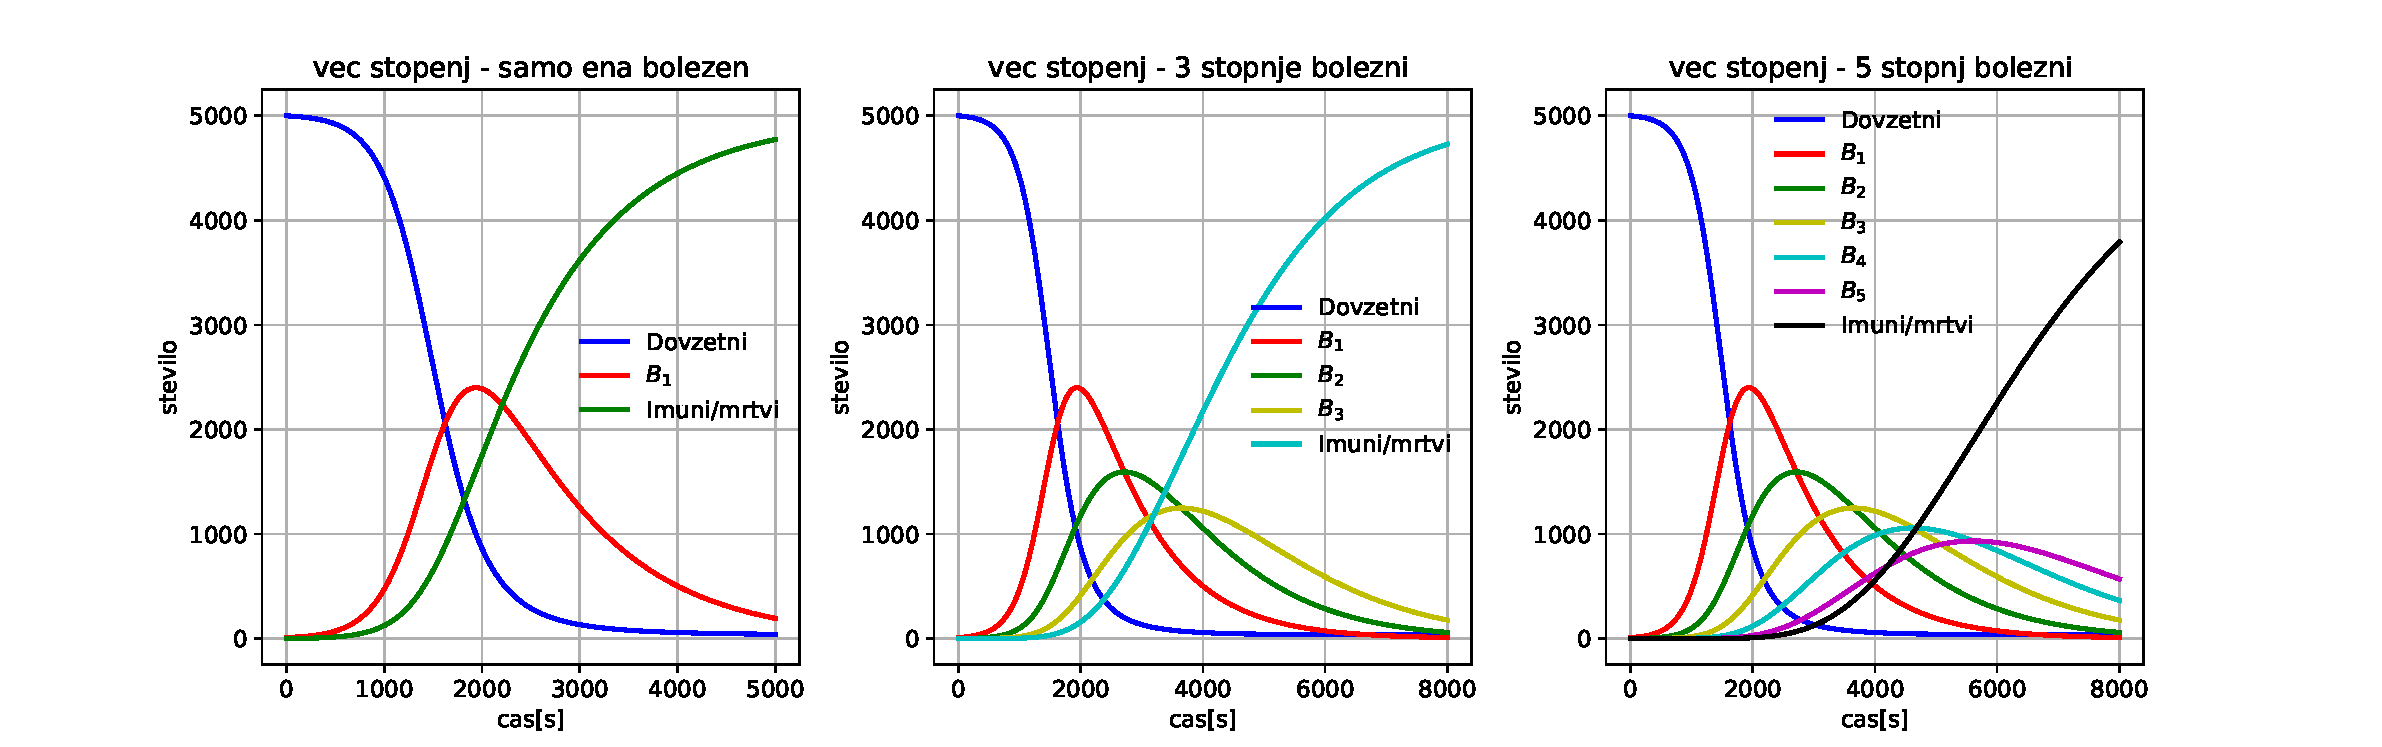
\includegraphics[width=22cm]{stopnjevanje_bolezni.pdf}
  \caption{Več stopenj bolezni omili končni razmah epidemije toda podaljša čas trajanja epidemije. V limiti veliko stopenj bi tako epidemija propadla, bolezen pa se nebi razširila.}
\end{figure}

\section{Model Lotka-Volterra}
Oglejmo si sedaj model plenilec - plen, ki ga prav tako opišemo s logističnim modelom:


\begin{equation}
\begin{array} {lcl} \dot{Z} & = & +\alpha Z - \beta ZL \\
\dot{L}  & = &  -\gamma L + \delta ZL   \\
 \end{array}
\end{equation}
Z uvedbo brezdimenzijskega časa $\tau = t \sqrt{\alpha \gamma}$, brezdim. lisic $l = \frac{\beta}{\alpha}L$ in zajcev $z = \frac{\delta}{\gamma} Z$ lahko sistem prevedemo le na eno parametrični sistem enačb: 
\begin{equation}
\begin{array} {lcl} \dot{z} & = & +p z(1-l) \\
\dot{l}  & = & \frac{l}{p}(z-1)\\
 \end{array}
\end{equation}
, kjer je $p = \sqrt{\frac{\alpha}{\gamma}}$ in pove razmerje rojevanja zajcev proti umiranju lisic.
\subsection{Oscilacije zajcev in lisic}
Ko numerično integriramo enačbe (4) dobimo naslednjo oscilacije populacij, sepravi ko naraste število zajcev, naraste tudi število lisic, ki pobijejo zajce in nato tudi same umrejo. Perioda oscilacij je odvisna od začetne populacije zajcev in lisic ter paramtera p.
\begin{figure}[htb!]
  \centering
  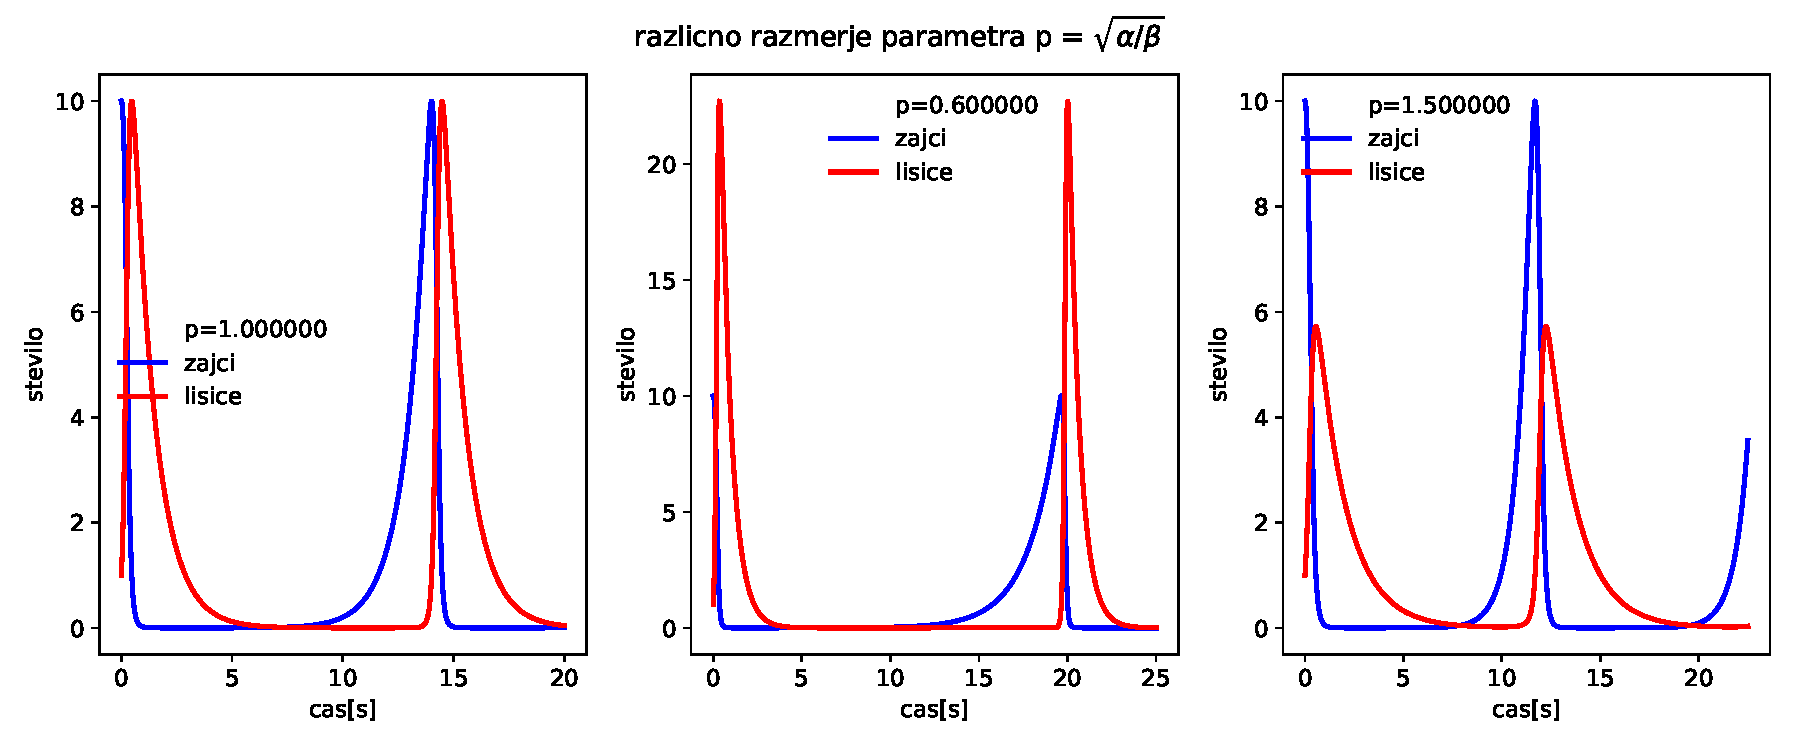
\includegraphics[width=18cm]{zajci_razlicna_razmerja.pdf}
  \caption{Periode se z naraščanjem p krajšajo saj se zajci hitreje razmahnejo in postanejo na voljo za razmah lisic.}
\end{figure}

\begin{figure}[htb!]
  \centering
  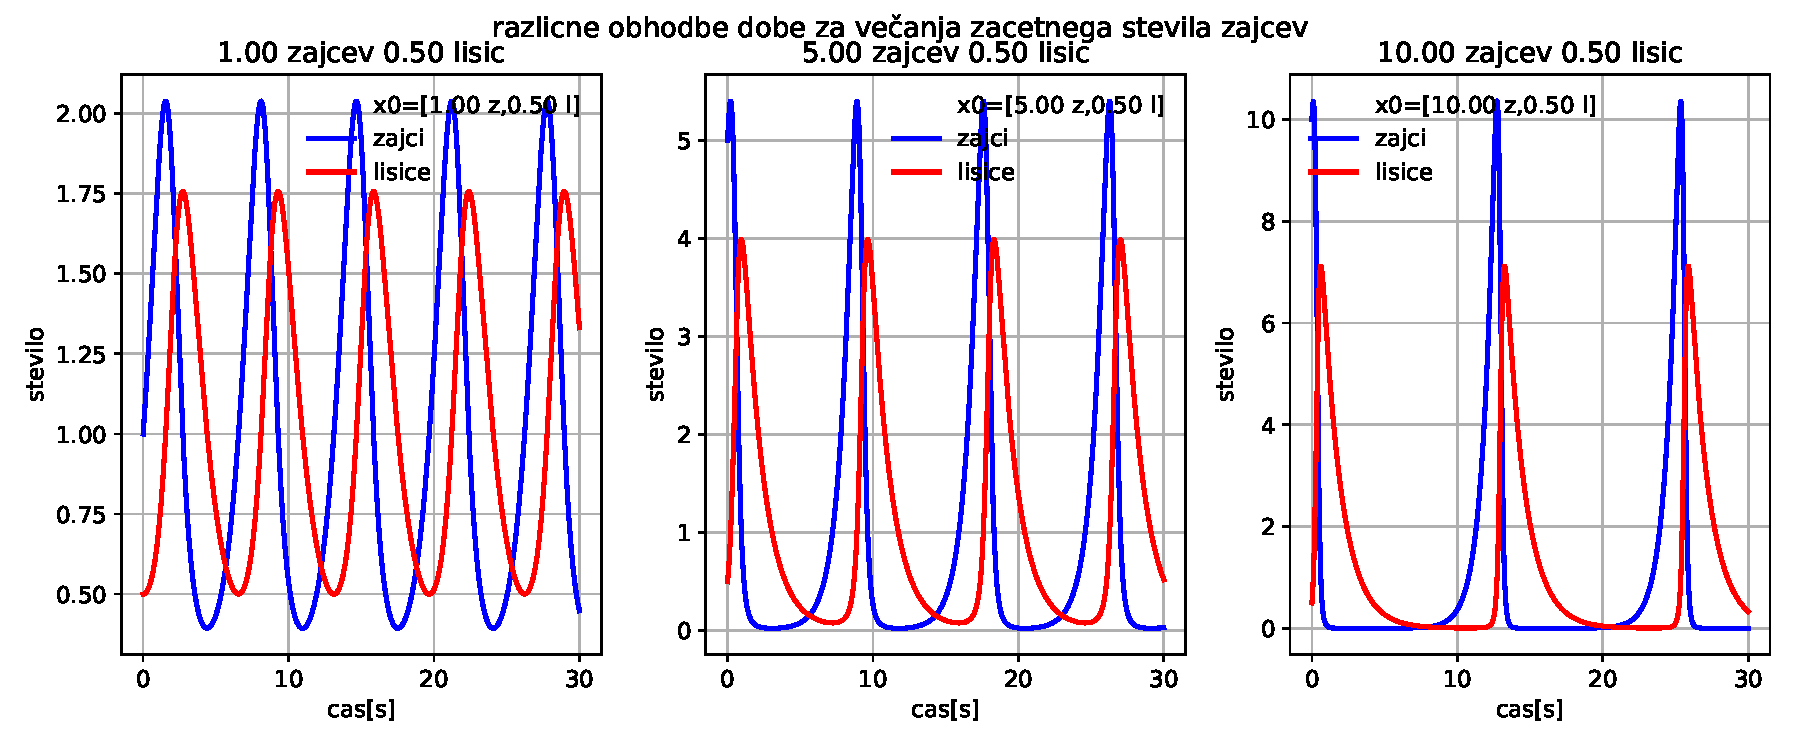
\includegraphics[width=18cm]{zajci_razlicni_zacetni_vecanje_zajci.pdf}
  \caption{Iz tega grafa vidimo da se pri manjšem začetnem številu zajcev in lisic naraščanje postane bolj milo in zvezno kot v zgornjem primeru. Periode se z večanjem začetnega števila zajcev krajšajo, prav tako pa se zviša maksimum obeh populacij.}
\end{figure}
\begin{figure}[htb!]
  \centering
  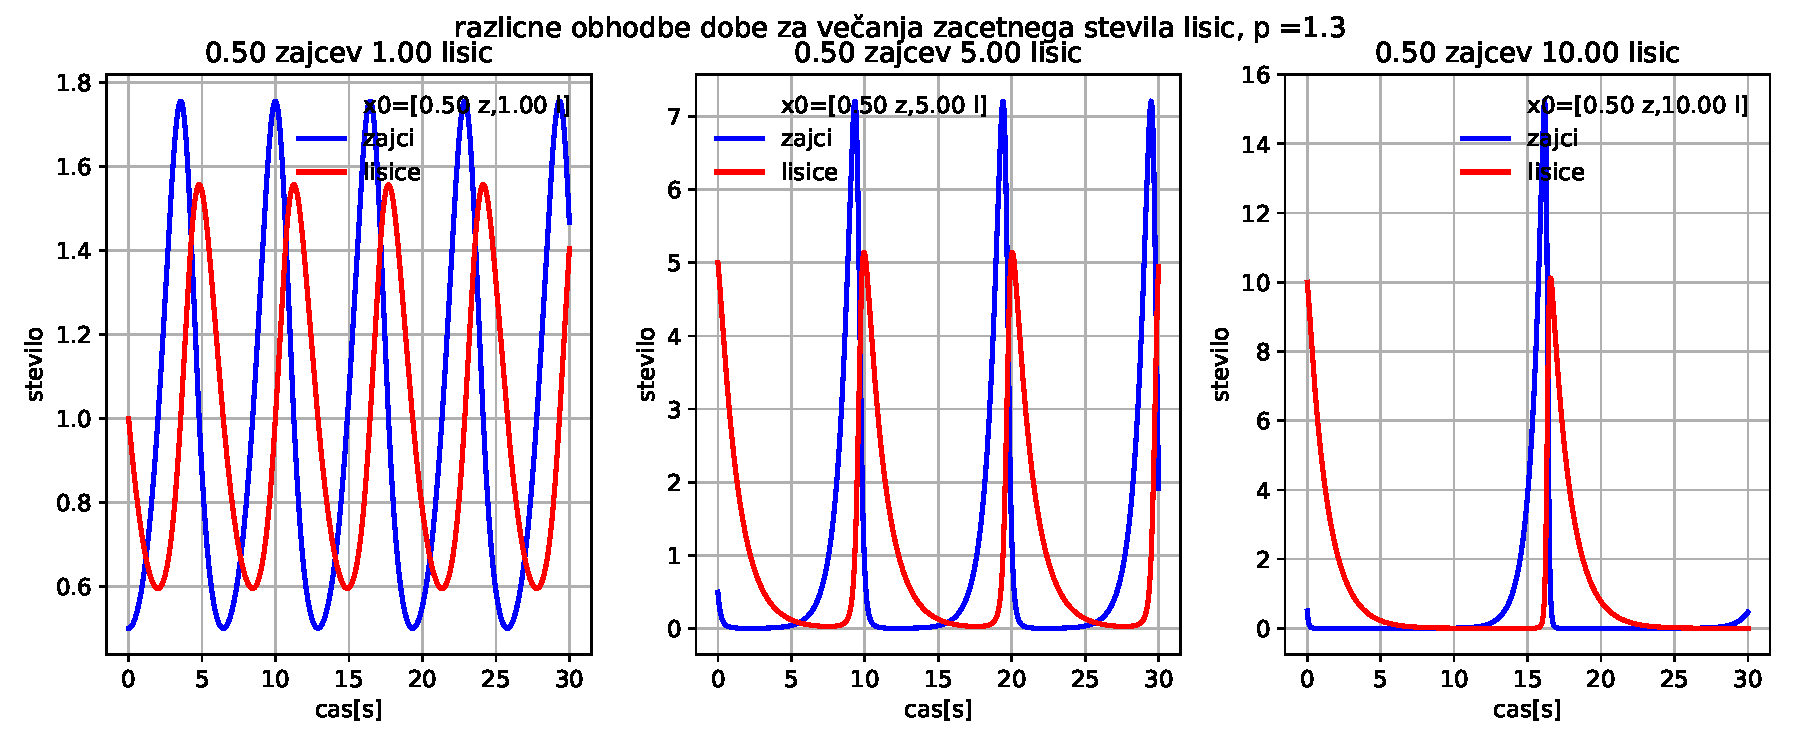
\includegraphics[width=18cm]{zajci_razlicni_zacetni_vecanje_lisic.pdf}
  \caption{Z večanjem lisic se podobno kot z večanjem zajcev daljša obhodna doba populacij, končno število zajcev pa se zanimivo MOČNO poveča??? (to mi ni čisto logično??..., ampak izgleda, da je parameter p = 1.3 v prid zajcem in jih zato nastane več, čeprav smo povečevali število lisic.}
\end{figure}


\begin{figure}[htb!]
  \centering
  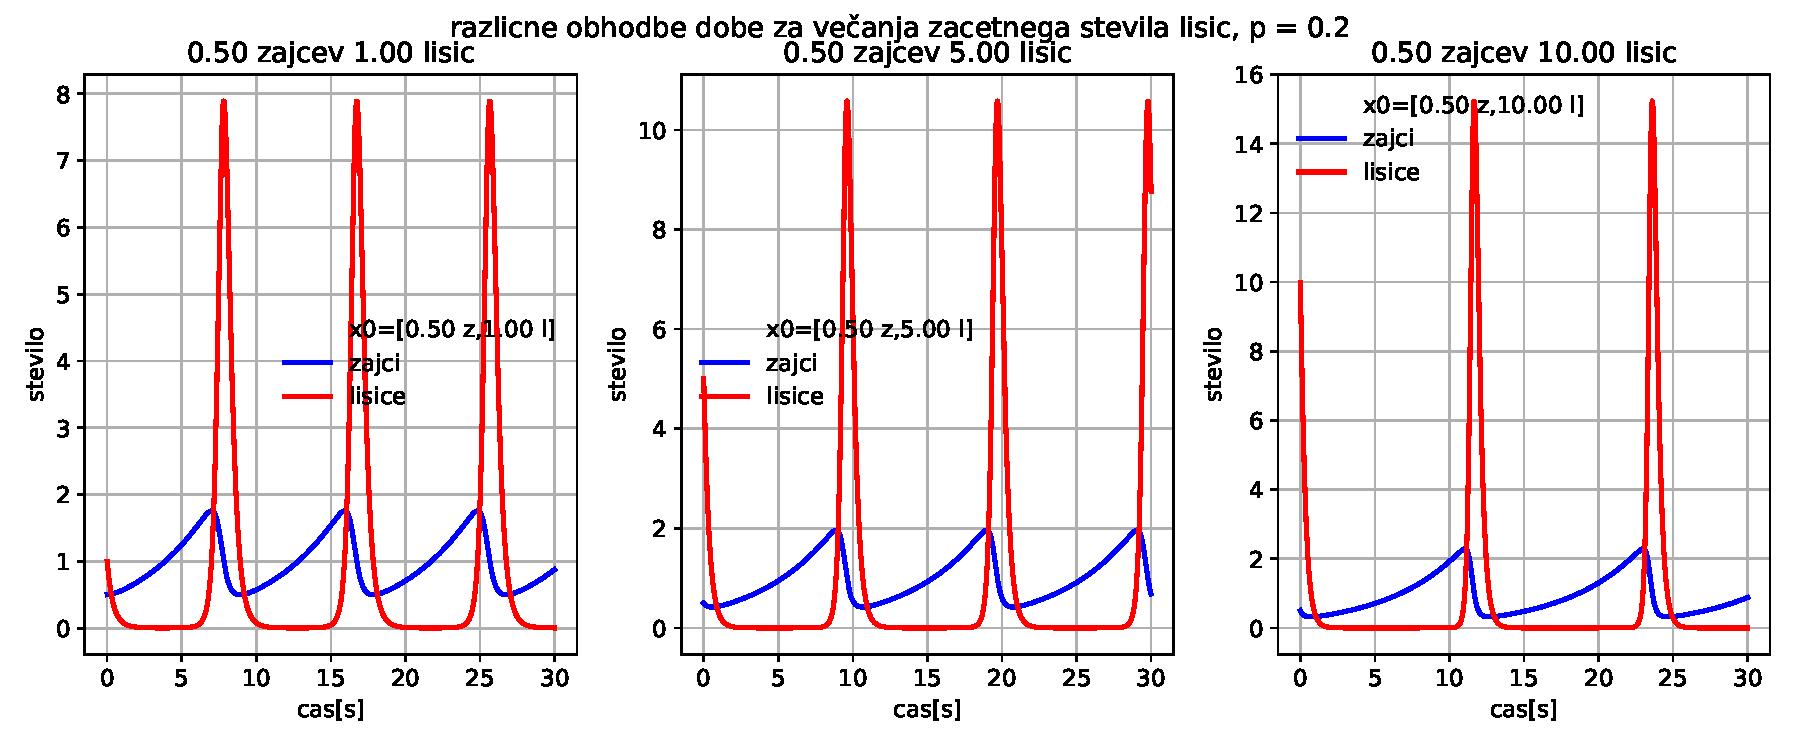
\includegraphics[width=18cm]{zajci_razlicni_zacetni_vecanje_lisic_bolj_realno.pdf}
  \caption{Če spremenimo razmerje rojevanja zajcev in umiranja lisic, dobimo manj zajcev in vedno enako število zajcev ne glede na število lisisc. To mi zopet ni nekako logično, ker imamo lahko večje število lisic tudi če je zajcev manj. Izgleda da čas hranjenja z zajci (i.e daljše obhodne dobe) omogočajo da v vsaki obhodni dobi nastane več lisic.}
\end{figure}


Integracijska shema nam pri nekaterih začetnih pogojih odpove. To se pogosteje dogaja pri velikih vrednostih $z(0),l(0),p$.\newpage
\begin{figure}[htb!]
  \centering
  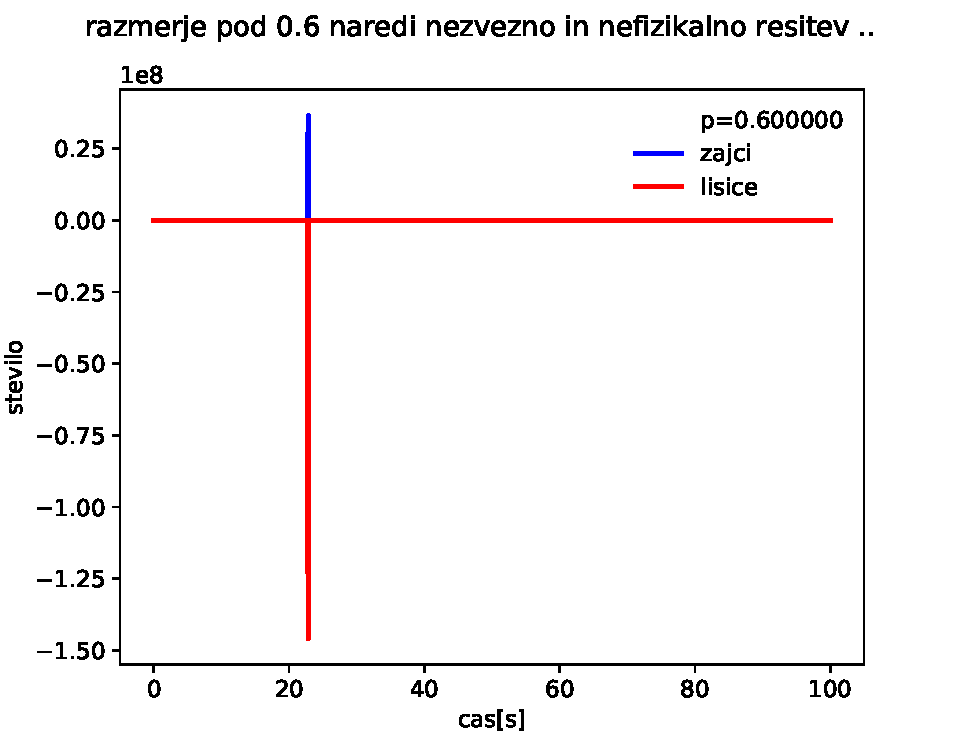
\includegraphics[width=10cm]{zajci_nefizikalna_resitev.pdf}
  \caption{Odpoved integracijske sheme za nekatere začetne pogoje.}
\end{figure}
\subsection{Zastojne točke}
Zanima me ali obstajajo posebne rešitve sistema enačb(4), ki jih imenujemo zastojne točke in so nekako podobne stacionarnem stanju pri PDE. Postavimo torej $\dot{z}, \dot{l}$ na $0$ in dobimo dve točki $(0,0)$ in $(1,1)$. Če vstavimo ti dve točki kot začetne pogoje v osnovni sistem (4), vidimo da se rešitev na teh točkah ne propagira ampak ostane tam, ker so tam vsi odvodi enaki 0. Te točke so lahko stabilne (kot nekakšna potencialna jama), tako da se vsaka rešitev propagira nazaj v točko, ali pa nestabilne in se rešitev nikoli več ne propagira v zastojno točko. To se lahko preuči s Jakobijevo determinanto ali pa pogleda na fazni digram, kot bomo storili na sliki 10. Če enačbo (4) razvijemo okoli točke $(0,0)$ dobimo razvoj sistema po prvem redu:
\begin{equation}
\begin{array} {lcl} \dot{z} & = & pz \\
\dot{l}  & = & -\frac{l}{p}\\
 \end{array}
\end{equation} 
Za razvoj okoli točke (1,1) pa dobimo:
\begin{equation}
\begin{array} {lcl} \dot{z} & = & -p l \\
\dot{l}  & = & \frac{z}{p}\\
 \end{array}
\end{equation} 
Stabilnost točke lahko preverimo če malo izmaknemo začetne pogoje:
\begin{figure}[htb!]
  \centering
  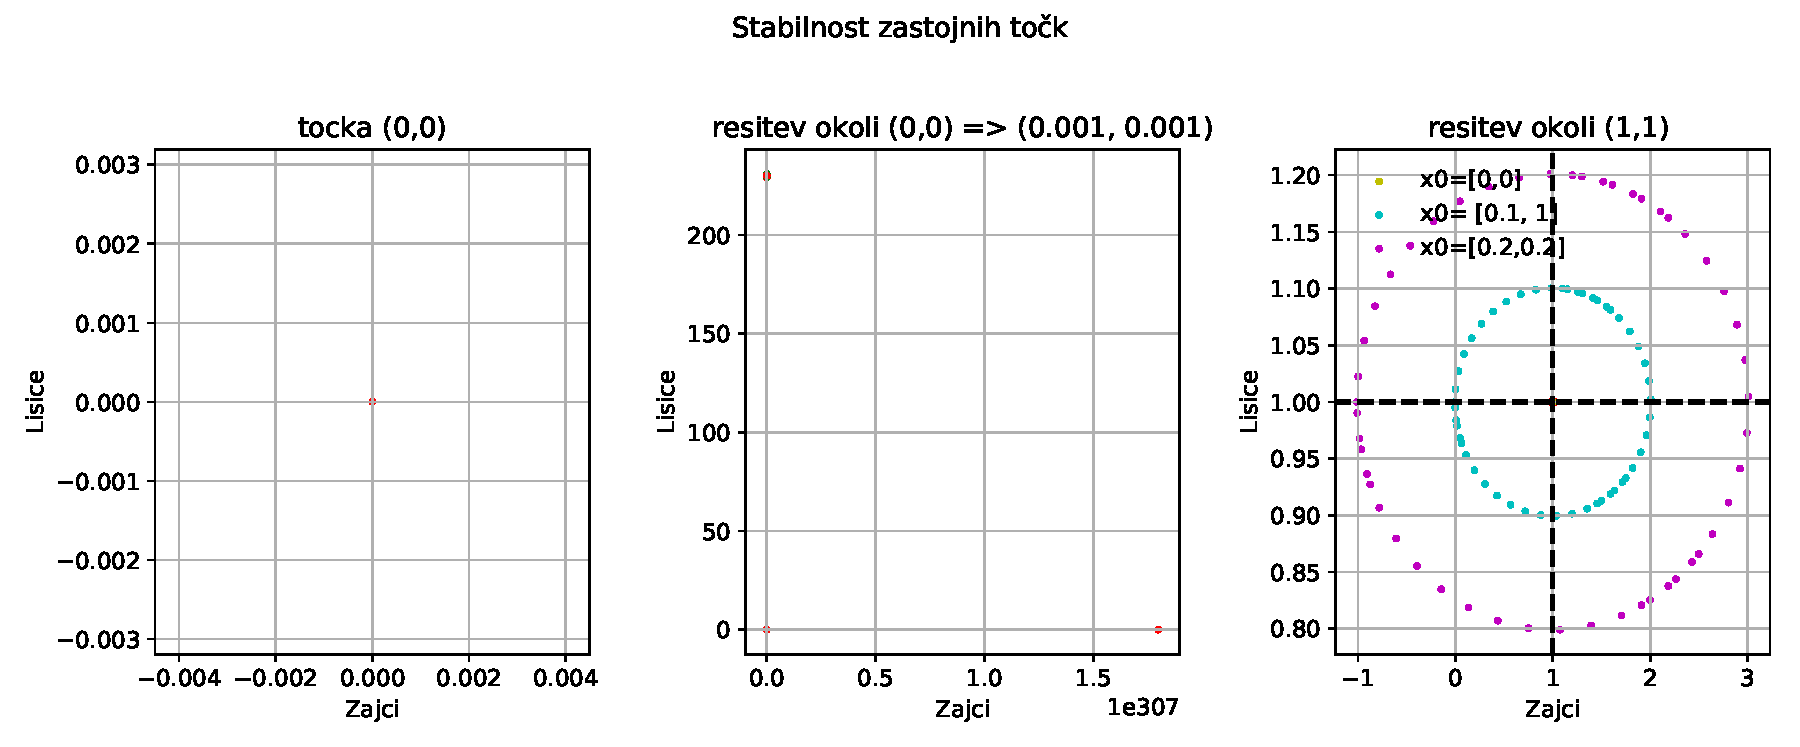
\includegraphics[width=18cm]{zajci_stabilnost1.pdf}
  \caption{Rešitev sistema enačb (5),(6). Kot je vidno je točka (0,0) nestabilna in tocka(1,1) tudi, saj se fazni diagram ne konča v njih.}
\end{figure}

Prava rešitev nam razvito rešitev - krožnico, s oddaljevanjem od točke točke (1,1) zmeraj bolj deformira.
\begin{figure}[h]
  \centering
 
  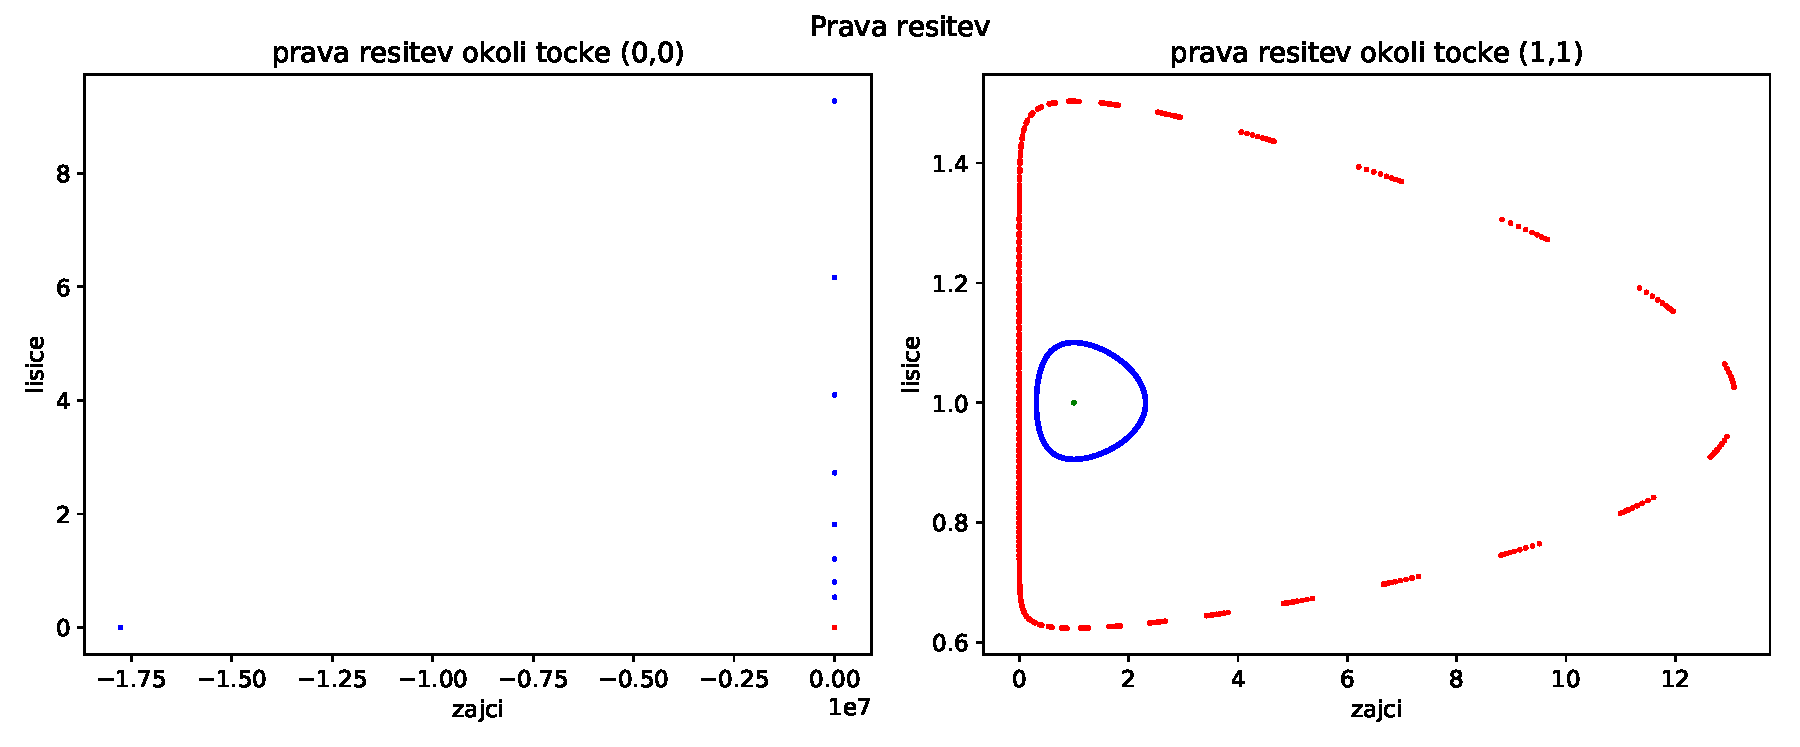
\includegraphics[width=17cm]{zajci_stabilnost1_prava.pdf}
  \caption{Vidimo da je v okolici zastojne točke (1,1) fazni diagram približno krožnica, vse bolj stran pa razvoj rešitve ni večdober. Rešitev okoli (0,0) pa nam odpove (integracijsko), tako kot na sliki 10.}
\end{figure}


\section{Laser - populacija fotonov}
Laser predstavlja koherentno svetlobo. Opišemo ga s modelom resonatorja, v katerem imamo fotone in vzbujene atome, ki jim fotoni povzročajo stimulirano emisijo, in tako atomi izsevajo nove fotone, ter se združijo s fotonom, ki vzbuja. Tako torej srečanje fotona z vzbujenim atomom zmanjšuje število vzbujenih atomov na časovno enoto v resonatorju. Prav tako atomi prehajajo v osnovne stanje s spontano emisijo, zato se njihovo število manjša, za fotone pa privzamemo da nekateri pobegnejo iz resonatorja.  
Zapišimo zopet sistem enačb za populacijo, kjer so $a$ število atomov, $f$ število fotonov in $Q$ črpanje atomov v resonator : 
\begin{equation}
\begin{array} {lcl} \dot{f} & = & -B f + D a f \\
\dot{a}  & = & -Ca + E af + Q \\
 \end{array}
\end{equation}
Ta sistem lahko zopet prepišemo v brezdimenzijsko obliko in tako prevedmo sistem na le dva prosta parametra.
\begin{equation}
\begin{array} {lcl} \dot{F} & = & \frac{F}{p} (A-1) \\
\dot{A}  & = & q - p A (F+1) \\
 \end{array}
\end{equation}
Zastojni točki sta $(\frac{q}{p},0)$ in $(q, \frac{q}{p}-1)$.
Za razmah laserja mora biti $q > p$, torej črpanje močnejše od umiranja atomov, kar se tudi vidi iz rešitve:

\begin{figure}[htb!]
  \centering
  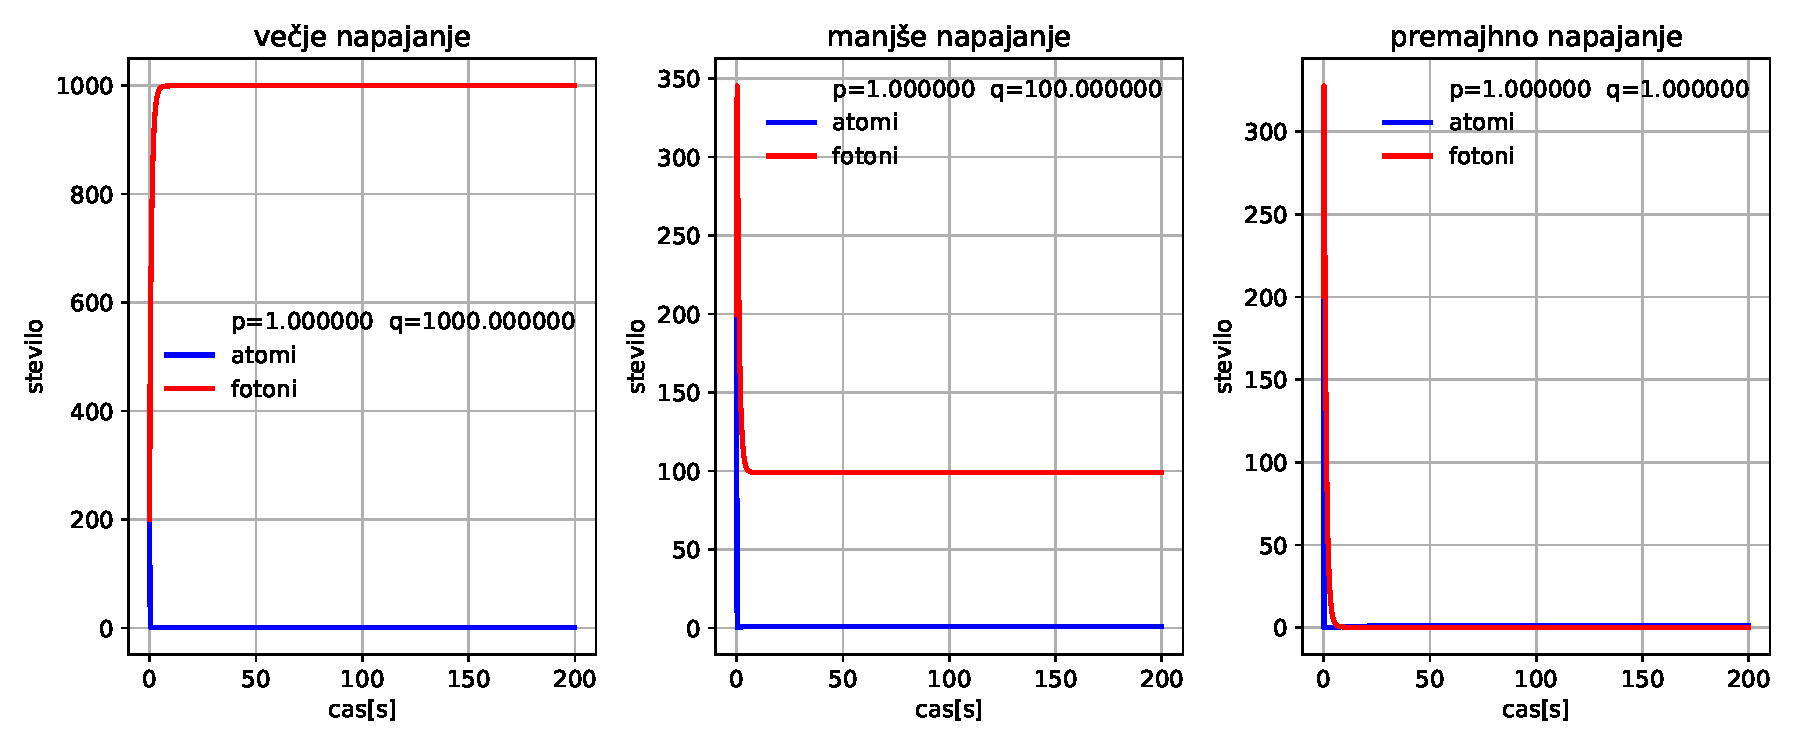
\includegraphics[width=18cm]{laser_razlicno_napajanje.pdf}
  \caption{Različno močno napajanje nam vpliva na končno število fotonov. Če je napajanje premajhno ne bomo imeli fotonov v resonatorju, saj bodo vsi atomi razpadli hitreje kot jih bomo dovajali. }
\end{figure}
Zgornji režim ne vsebuje oscilacij zaradi visokih vrednosti paramterov. Če te postavimo na manjše vrednosti dobimo nov režim - oscilacije pred stacionarim stanjem.\newline\newline
To lahko opazujemo tudi na faznem diagramu

\begin{figure}[htb!]
  \centering
  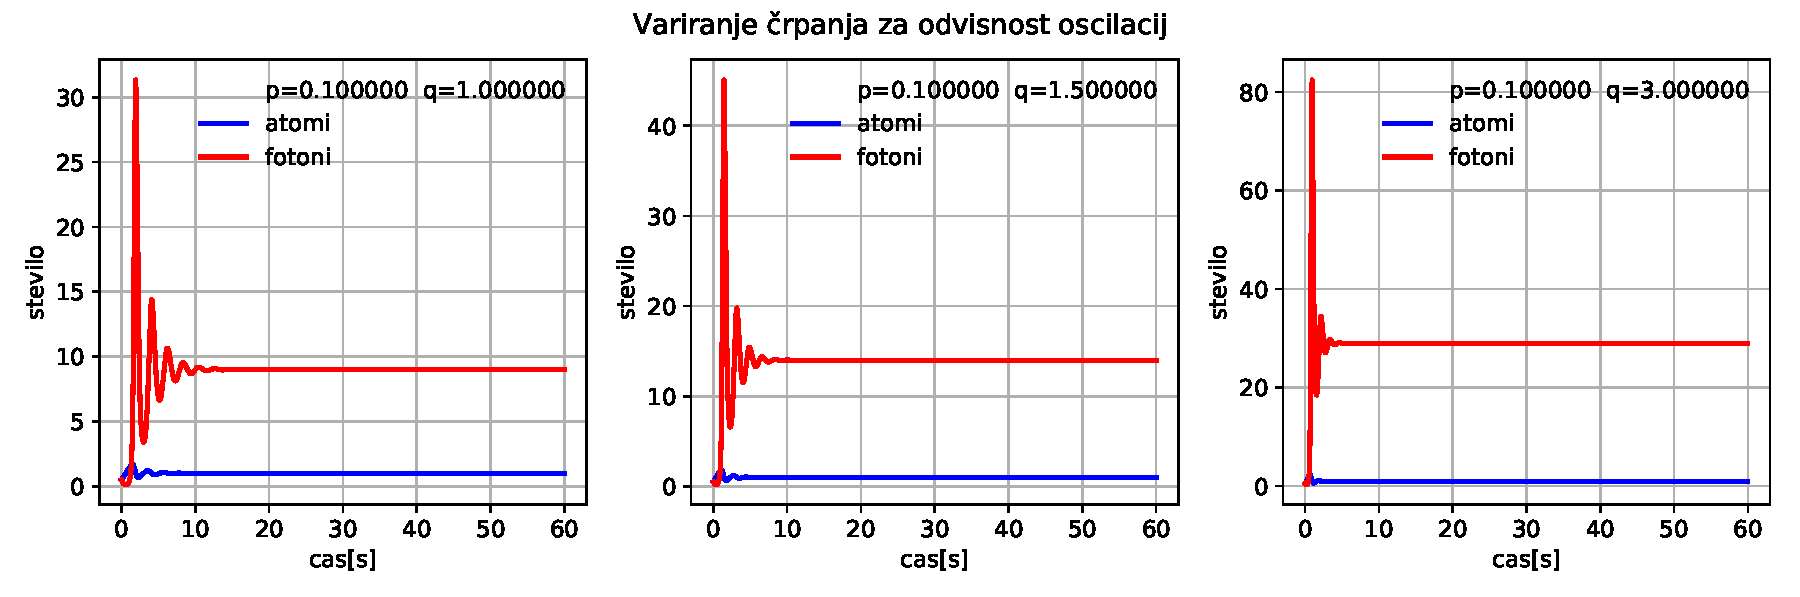
\includegraphics[width=18cm]{laser_oscilacije_crpanje.pdf}
  \caption{Vidimo, da je relaksacijski čas s večjim črpanjem krajši, oscialcije večja in frekvenca oscialcij večja. Vidi se tudi da je razmerje ravnovesnega števila fotonov približno $\frac{q}{p}$. Število atomov pa bo v primeru razvoja fotonov zelo nizko, saj v vsakem trenutku črpane atome izločimo prek vzbuditve in izsevanja novega fotona.  }
\end{figure}


\begin{figure}[htb!]
  \centering
  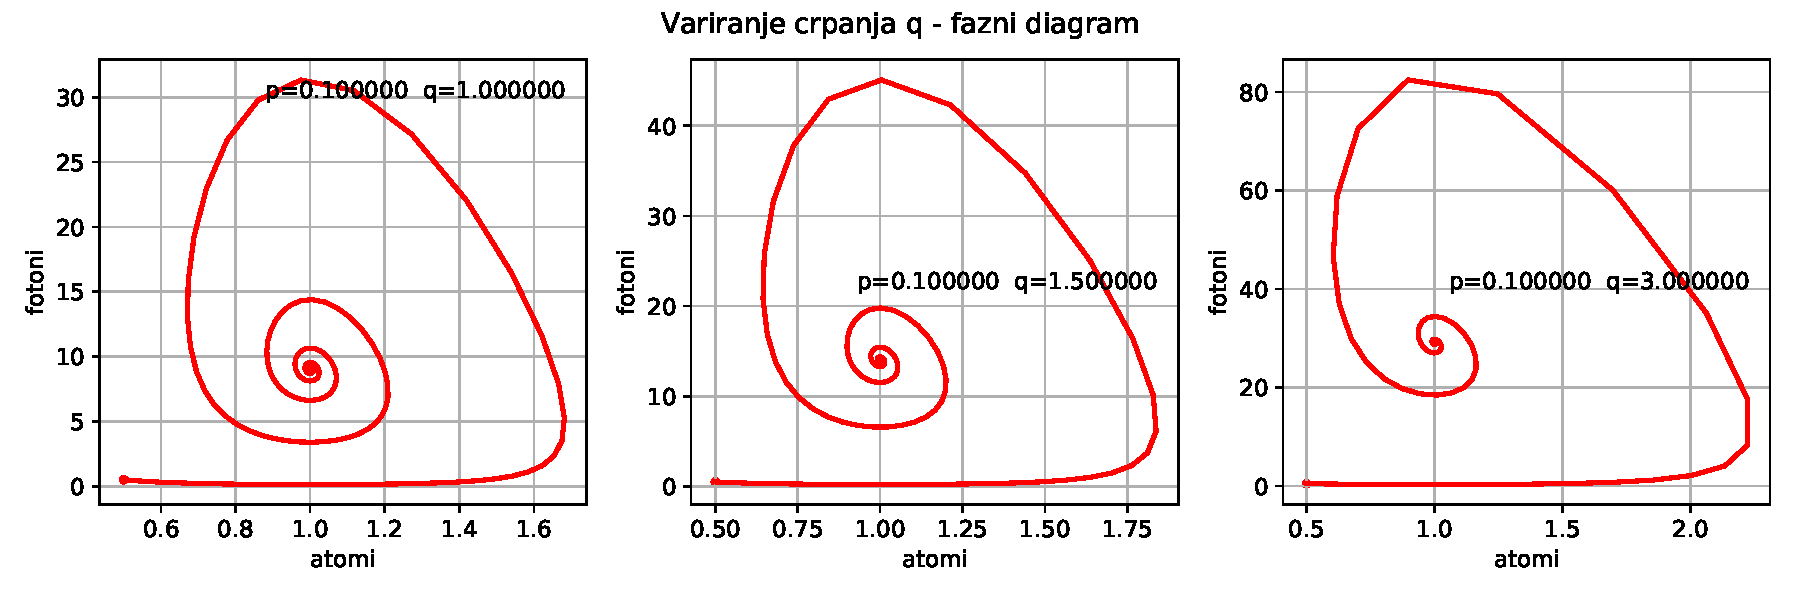
\includegraphics[width=18cm]{laser_oscilacije_crpanje_fazni_diagram.pdf}
  \caption{Fazni diagram, kjer se vidi spiralsta ravnovesna oblika in pa večanje amplituide oscialcij ter več period/obhodov (bolj zavita spirala) pri manjšem črpanju.}
\end{figure}

\subsection{Zastojni točki}
Zanima nas ali sta astojni točki $A =(a,f)= (\frac{q}{p},0)$ in $ B= (q, \frac{q}{p}-1)$ stabilni ali nestabilni. Iz slike(12) je očitno, da obstaja stabilna točka, vendar le v določenih pogojih in sicer, ko je laser v delujočem režimu in je $q>p$, se laser vedno ustali na točki $(a,f) = (1, q/p - 1)$.
Točka $A =  (\frac{q}{p},0)$, pa je nestabilna , torej v režimu $q>p$ laser nima stacionarnega stanja, razen v eni točki, ko je število fotonov nič.


\begin{figure}[htb!]
  \centering
  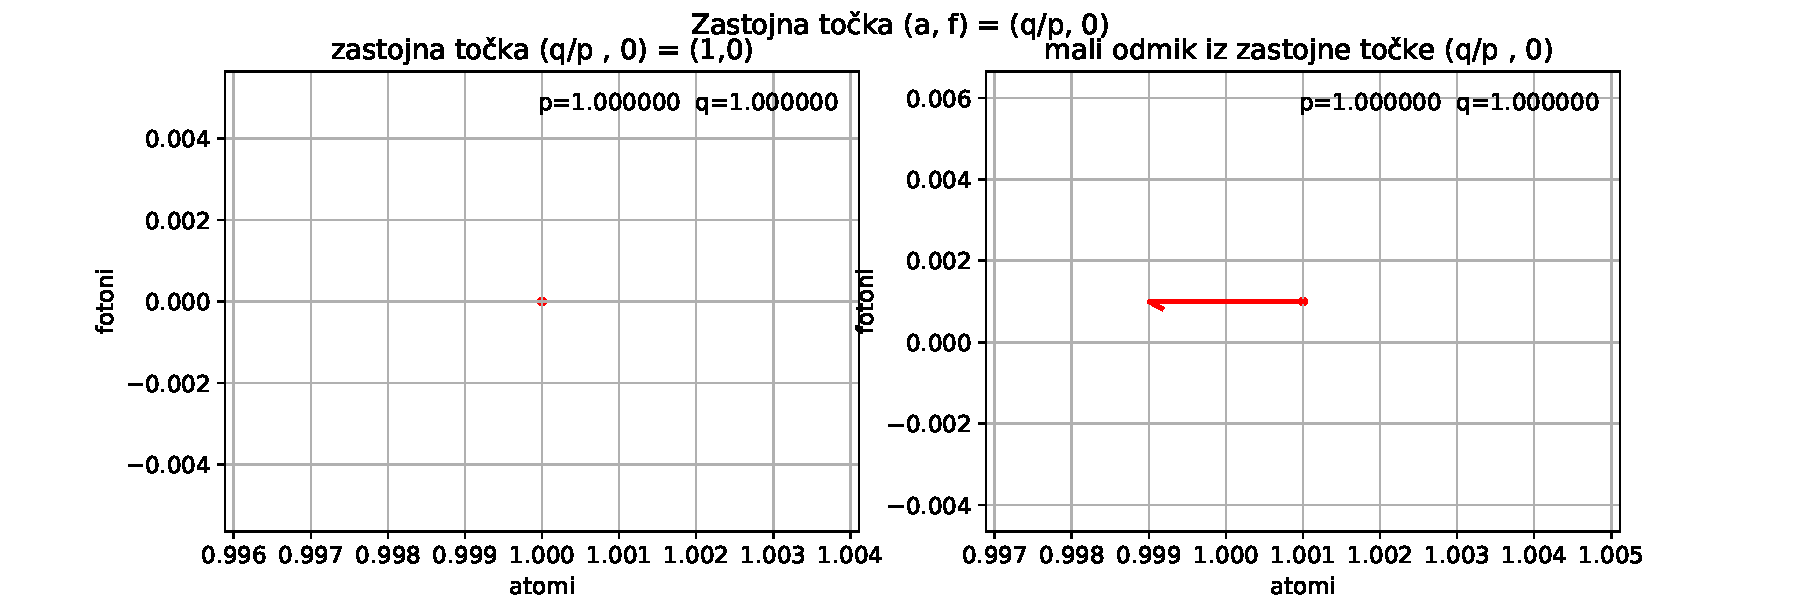
\includegraphics[width=18cm]{laser_zastojna_tocka_1.pdf}
  \caption{Izmik iz zastojne točke $A =(a,f)= (\frac{q}{p},0) = (1,0)$ nam pokaže, da ta točka ni stabilna.}
\end{figure}

\begin{figure}[htb!]
  \centering
  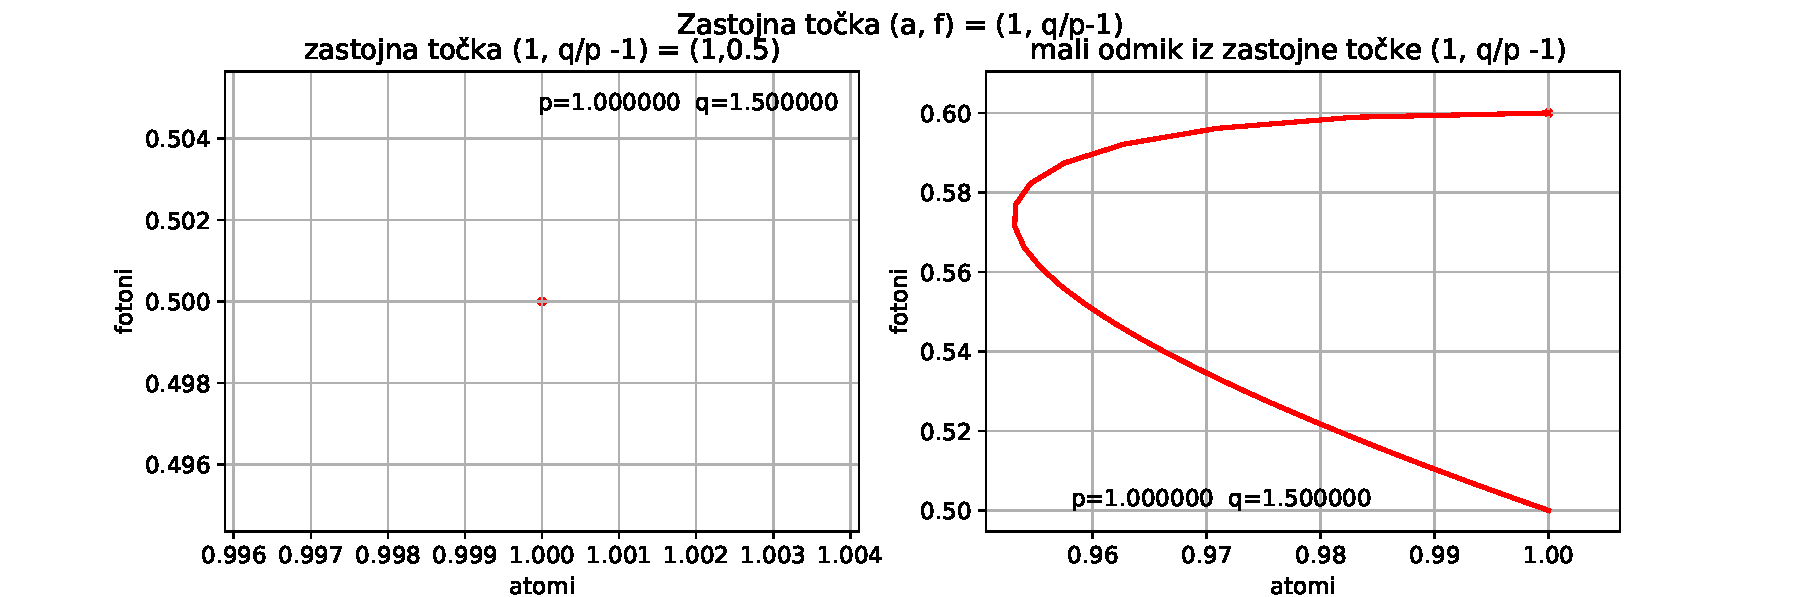
\includegraphics[width=18cm]{laser_zastojna_tocka_2.pdf}
  \caption{Izmik iz druge zastojne točke pa nas vedno vrne nazaj v zastojno točko, torej gre za edino stabilno točko v naših problemih.}
\end{figure}

\end{document}